\chapter{Implementation}
\label{ch:implementation}

This chapter describes the implementation of the system, it is divided into two parts.
The first part describes the interaction between the Raspberry Pi and the devices connected to it.
The second part is about the interaction between the client and the Raspberry Pi.

% -----------------------------------------------------------------------------
\section{Devices}
\label{ch:implementation:sec:devices}

To manage the devices connected to the Raspberry Pi, the library WiringPi~\cite{WiringPi} is used with a shield to plug adapters on the Raspberry Pi.
Referring to the figure \ref{fig:analysis:communication:illustration}, the Raspberry Pi must have 4-20mA and 1-5V adapters.
These device adapters are connected to the Raspberry Pi with the shield and the protocol is I2C~\cite{i2c} and SPI~\cite{spi}.

\subsection{1-5V sensor}
\label{ch:implementation:sec:devices:subsec:i2c}

To read the 1-5V, we need to use the ADC 8 Click \ref{fig:analysis:mcu:1-5V}.
This device use I2C protocol which is a serial communication.
This is a master-slave protocol, the master is the Raspberry Pi and the slaves are the devices connected to the Raspberry Pi.
The master is the only one that can initiate a communication, the slaves can only respond to the master.
The master can communicate with multiple slaves, but the slaves can only communicate with the master.
The communication is done with two wires, one for the clock and one for the data.
The clock is generated by the master and the data is sent by the master or the slave depending on the direction of the communication.

\subsubsection{Setup}
\label{ch:implementation:sec:devices:subsec:1-5V:setup}

To use I2C on the Raspberry Pi, the I2C interface must be enabled.

\begin{code}
  \captionof{listing}{Enable I2C on the Raspberry Pi}
  \label{code:implementation:sec:devices:1-5V:setup}
  \begin{minted}{bash}
      sudo raspi-config
      # Select Interfacing Options
      # Select I2C
      # Select Yes
      # Select Ok
      # Select Finish
      sudo reboot
  \end{minted}
\end{code}

As shown in the code \ref{code:implementation:sec:devices:1-5V:setup}, the I2C interface is enabled in the Raspberry Pi configuration and he must

\subsubsection{Example}
\label{ch:implementation:sec:devices:subsec:1-5V:example}

To use the ADC 8 Click\ref{fig:analysis:mcu:1-5V}, it's possible to use the single header file Adafruit\_ADS1X15.h~\cite{ads1x15}.
This file is a version of the library provided by Adafruit adapted for the Raspberry Pi with using WiringPi~\cite{WiringPi}.
The following code \ref{code:implementation:sec:devices:subsec:1-5V:example} is an example of how to read data from the ADC 8 Click.

\begin{code}
  \captionof{listing}{Example of reading data from the ADC 8 Click}
  \label{code:implementation:sec:devices:subsec:1-5V:example}
  \begin{minted}{c++}
#include <stdio.h>
#include <unistd.h>
#include "includes/ADS1X15/Adafruit_ADS1X15.h"

void printBits(size_t const size, void const* const ptr);

Adafruit_ADS1115 ads;

int main(int argc, char* argv[]) {
    int16_t adc0;
    double milliVolts;
    double bits2milliVoltsFactor;

    // The ADC input range (or gain) can be changed via the
    // following functions, but be careful never to exceed
    // VDD +0.3V max, or to exceed the upper and lower limits
    // if you adjust the input range! Setting these values
    // incorrectly may destroy your ADC!
    //                               ADS1015  ADS1115
    //                               -------  -------
    // 2/3x gain +/- 6.144V  1 bit = 3mV      0.1875mV (default)
    // 1x gain   +/- 4.096V  1 bit = 2mV      0.125mV
    // 2x gain   +/- 2.048V  1 bit = 1mV      0.0625mV
    // 4x gain   +/- 1.024V  1 bit = 0.5mV    0.03125mV
    // 8x gain   +/- 0.512V  1 bit = 0.25mV   0.015625mV
    // 16x gain  +/- 0.256V  1 bit = 0.125mV  0.0078125mV
    ads.setGain(GAIN_ONE);
    // remember to change this according to gain
    bits2milliVoltsFactor = 0.125;

    ads.begin();
    while (true) {
        adc0 = ads.readADC_Differential_2_3();
        milliVolts = adc0 * bits2milliVoltsFactor;
        printBits(sizeof(adc0), &adc0);
        printf(" *** %5d *** %f\n", adc0, milliVolts);
        usleep(1000000);
    }
}

//assumes little endian
void printBits(size_t const size, void const* const ptr) {
    unsigned char* b = (unsigned char*)ptr;
    unsigned char byte;
    int i, j;

    for (i = size - 1; i >= 0; i--) {
        for (j = 7; j >= 0; j--) {
            byte = (b[i] >> j) & 1;
            printf("%u", byte);
        }
    }
}
  \end{minted}
\end{code}

\subsubsection{Electrical scheme}
\label{ch:implementation:sec:devices:subsec:1-5V:electrical-scheme}

The sensor is powered by a 10V to 24V power supply and provide a 1-5V output.
The ADC 8 Click\ref{fig:analysis:mcu:1-5V} can only read the voltage from 0 to Vcc + 0.3V.
By default, the jumper ont the ADC 8 Click is set to 3.3V, so the maximum voltage that can be read is 3.6V.
To transform the voltage from 1-5V to a range of 0-3.6V, a tension divider is used.

\begin{figure}[H]
  \centering
  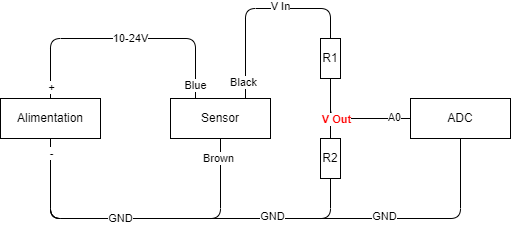
\includegraphics[width=1\textwidth]{img/implementation_tensionDivider.drawio.png}
  \caption{Electrical scheme of the 1-5V sensor}
  \label{fig:implementation:sec:devices:subsec:1-5V:electrical-scheme}
\end{figure}

The figure \ref{fig:implementation:sec:devices:subsec:1-5V:electrical-scheme} show the electrical scheme of the 1-5V sensor with a tension divider.
The V out of the tension divider can be calculated with the following formula:

\begin{figure}[ht]
  \centering
  \[ V_{out} = \frac{V_{in} \times R_1}{R_1 + R_2} \]
  \caption{Formula to calculate the V out of the tension divider}
  \label{fig:implementation:sec:devices:subsec:1-5V:electrical-scheme:formula}
\end{figure}

The following code \ref{code:implementation:sec:devices:subsec:1-5V:electrical-scheme:formula}
will find the best values for R1 and R2 assuming that the input voltage is 5V, the output voltage is 3.5V and
R1 + R2 \~= 10-20kOhm using the formula \ref{fig:implementation:sec:devices:subsec:1-5V:electrical-scheme:formula}:

\begin{code}
  \captionof{listing}{Formula to calculate the V out of the tension divider}
  \label{code:implementation:sec:devices:subsec:1-5V:electrical-scheme:formula}
  \begin{minted}{python}
possible_resistors = [3300,  4700,  5600,  6800, 8200,
                      10000, 12000, 15000, 18000]
max_vin = 5.0
max_vout = 3.5
min_r = 10000
max_r = 20000
possible_coupling = []


def compute_resistance(vin, r1, r2):
    return (vin * r1) / (r1 + r2)


def find_resistors():
    for r1 in possible_resistors:
        for r2 in possible_resistors:
            if min_r <= r1 + r2 <= max_r:
                vout = compute_resistance(max_vin, r1, r2)
                if vout <= max_vout:
                    possible_coupling.append((r1, r2, vout))

    return possible_coupling


def print_resistors(nb):
    for i in range(nb):
        print("R1: " + str(possible_coupling[i][0]) +
             " R2: " + str(possible_coupling[i][1]) +
             " Vout: " + str(
            possible_coupling[i][2]))


def main():
    couples = find_resistors()
    couples.sort(key=lambda x: x[2], reverse=True)
    print_resistors(5)


if __name__ == "__main__":
        main()
  \end{minted}
\end{code}

The goal is to find the couple of resistors that will give us the greater $V_{out}$ which is lower than the max allowed.
According to the situation that the max $V_{in}$ is 5V, the max $V_{out}$ is 3.5V and the couple of resistors must be between 10kOhm and 20kOhm.
The five best couples of resistors are those in the following table \ref{table:implementation:sec:devices:subsec:1-5V:electrical-scheme:formula}:

\begin{table}[H]
  \centering
  \begin{tabular}{|l|l|l|l|}
    \hline
    \texttt{R1} & \texttt{R2} &\texttt{$V_{out}$} & \texttt{R1 + R2} \\ \hline
    12000 & 5600 & 3.409 & 17600   \\ \hline
    10000 & 4700 & 3.401 & 14700   \\ \hline
    6800  & 3300 & 3.366 & 10100   \\ \hline
    10000 & 5600 & 3.205 & 15600   \\ \hline
    12000 & 6800 & 3.191 & 18800   \\ \hline
  \end{tabular}
  \caption{Best couples of resistors}
  \label{table:implementation:sec:devices:subsec:1-5V:electrical-scheme:formula}
\end{table}



\subsection{4-20mA controller}
\label{ch:implementation:sec:devices:4-20mA}

The 4-20mA sensor wasn't implemented during this project due to the lack of time.
The 4-20mA T 2 Click\ref{fig:analysis:mcu:4-20mA} is a 4-20mA current loop sender that uses SPI to communicate with the Raspberry Pi.
The SPI protocol is a synchronous serial communication interface specification used for short-distance communication, primarily in embedded systems.
Like the I2C, the SPI must be enabled on the Raspberry Pi.

\subsubsection{Setup}
\label{ch:implementation:sec:devices:4-20mA:setup}

To enable the SPI on the Raspberry Pi, the following steps must be done:

\begin{code}
  \captionof{listing}{Enable SPI on the Raspberry Pi}
  \label{code:implementation:sec:devices:4-20mA:setup}
  \begin{minted}{bash}
    sudo raspi-config
    # Select Interfacing Options
    # Select SPI
    # Select Yes
    # Select Finish
    sudo reboot
  \end{minted}
\end{code}

The code \ref{code:implementation:sec:devices:4-20mA:setup} is very similar to the code \ref{code:implementation:sec:devices:1-5V:setup} to enable the I2C.

\subsubsection{Electrical scheme}
\label{ch:implementation:sec:devices:4-20mA:electrical-scheme}

Like the 1-5V sensor, the 4-20mA controller need to have a alimentation from 10V to 24V.
The figure \ref{fig:implementation:sec:devices:subsec:4-20mA:electrical-scheme} show the electrical scheme of the 4-20mA controller:

\begin{figure}[H]
  \centering
  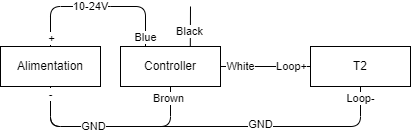
\includegraphics[width=1\textwidth]{img/implementation_4-20ma.drawio.png}
  \caption{Electrical scheme of the 4-20mA controller}
  \label{fig:implementation:sec:devices:subsec:4-20mA:electrical-scheme}
\end{figure}

As shown in the schema, the actual value isn't used by the Raspberry Pi because we can only send the data through the 4-20mA current loop.


\subsection{Serial rotary valve}
\label{ch:implementation:sec:devices:serial}

The rotary valve is a device that can open or close multiple holes by rotating a wheel.
This device is controlled by a serial communication.
To communicate with from the Raspberry Pi to the rotary valve, a USB to serial adapter is used.

\subsubsection{Setup}
\label{ch:implementation:sec:devices:serial:setup}

Like all the other devices, the serial communication must be enabled on the Raspberry Pi.
The following code \ref{code:implementation:sec:devices:serial:setup} show how to enable the serial communication:

\begin{code}
  \captionof{listing}{Enable serial communication on the Raspberry Pi}
  \label{code:implementation:sec:devices:serial:setup}
  \begin{minted}{bash}
    sudo raspi-config
    # Select Interfacing Options
    # Select Serial
    # Select No
    # Select Yes
    # Select Finish
    sudo reboot
  \end{minted}
\end{code}

\subsubsection{Usage}
\label{ch:implementation:sec:devices:usage}

The project contains a class RVM that is used to control the rotary valve.
This class is simply the utilization of the rotary valve.
This code \ref{code:implementation:sec:devices:usage} show how to use the RVM class:

\begin{code}
  \captionof{listing}{Usage of the RVM class}
  \label{code:implementation:sec:devices:usage}
  \begin{minted}{c++}
// On top of the main
wiringPiSetup();
// Initialization
RvmSetup rvmSetup{.device = "/dev/ttyUSB0"};
RVM rvm{Slot::No, rvmSetup};
rvm.start();
// Usage
rvm.moveTo(3);
  \end{minted}
\end{code}

\subsubsection{Add a new action}
\label{ch:implementation:sec:devices:add-action}

During the next steps of the project, the rotary valve will be used with new actions.
To add a new action, several steps must be done.

First of all, the new action will a new function in the RVM class.
This function will be declared in the RVM.h file and implemented in the RVM.cpp file.

The second step is to send the action to the rotary valve through the serial communication.
The command sent to the rotary valve is to follow a specific format: \texttt{/ + 1 + command + R + <CR>}.
The '1' is the address of the rotary valve and the 'R' and the <CR> are the end of the command.

The third step is not mandatory but the function \texttt{waitUntilFinish()} can be useful if the action needs to be done before the next action.
This method read the state of the rotary valve and leave the loop when the action is done.


\subsection{Add a new device}
\label{ch:implementation:sec:devices:add-device}
This project is designed to be easily extendable.
To add a new device, several steps must be done.

\begin{itemize}
  \item Create a new class in the \texttt{devices} folder. This class must inherit from the \texttt{Device} class.
  \item Create a new setup class in the same file. This class will be used to store the settings of the device that will be used at the initialization.
  \item Implement all the virtual methods of the \texttt{Device} class.
  \item Implement the method specific to the device.
\end{itemize}

To use this new device, you must create a new instance of the setup class and pass it to the constructor of the device.
The device contains a method \texttt{start()} that must be called to enable the device.
The following code \ref{code:implementation:sec:devices:add-device} show an example of the creation of the fan:

\begin{code}
  \captionof{listing}{Add a new device}
  \label{code:implementation:sec:devices:add-device}
  \begin{minted}{c++}
// Creation of the setup instance
FanSetup fanSetup{.pin = 28};
// Create the device with the setup
Fan fan{Slot::No, fanSetup};
// Enable the device
fan.start();
// Use the device
fan.off();
  \end{minted}
\end{code}


\section{Communications}
\label{ch:implementation:sec:communications}

The communication between the Raspberry Pi and the client is done through a Web socket and a REST API.

\subsection{REST API}
\label{ch:implementation:sec:communications:rest-api}

The REST API is used by the client to send action to the Core application.
Sometimes, the response is directly sent to the client in HTTP response but the most of the time, the response is sent through the Web socket.

\subsubsection{Core application}
\label{ch:implementation:sec:communications:rest-api:core}

The core application is running a HTTP server that listens on the port 8080.
It uses the single header library \texttt{HTTPLib} to handle the HTTP request.
This library is overridden by the class \texttt{communication/rest} that manage \acrshort{cors} and log the request.
The explanation of the sequence to register and handle a route is explained in the section \ref{conception:core-application:register-routes}.

To register a route, the server must be initialized and use the method \texttt{bindGet/Post(route, method)}.
The route is the path of the request behind the host and the prefix (now: \texttt{/api/v1/}).
The method is a function that takes three arguments: the server, the request and the response.
The server is to be able to get the state of the application and interact with it.
The request is the HTTP request to send by the client and the response to modify the status code of the response.

The following code \ref{code:implementation:sec:communications:rest-api:core} show how to register a route with an existing function or a lambda:

\begin{code}
  \captionof{listing}{Register a route with an existing function}
  \label{code:implementation:sec:communications:rest-api:core}
  \begin{minted}{c++}
#include <stdio.h>
#include "src/rest/server.h"

std::string healthCheck(Server& svr,
                        const httplib::Request& req,
                        httplib::Response& res) {
  printf("Health check\n");
  auto i = Info::getInstance();
  return R"({"status": ")" + i->getStatus() + R"("})";
}

int main() {

  Server server{8080};

  // Bind an existing function
  server.bindGet("health", healthCheck);
  // lambda expression
  server.bindPost("move", [](Server& svr,
                             const httplib::Request& req,
                             httplib::Response& res) {
      return "Hello World!";
  });

  server.startListening();
  return 0;
}
  \end{minted}
\end{code}

To use a route in the client, the client must send a request using the package HTTP of the Flutter framework.
The following code \ref{code:implementation:sec:communications:rest-api:core-client} show how to send a request to the route \texttt{/api/v1/moveTo} with the position in the body:

\begin{code}
  \captionof{listing}{Send a request to the route /api/v1/health}
  \label{code:implementation:sec:communications:rest-api:core-client}
  \begin{minted}{dart}
import 'dart:convert';
import 'package:http/http.dart' as http;

class Api {
  Future<bool> moveTo(int position) async {
    // Fetch data from the internet
    final response = await http.post(
      Uri.parse('http://127.0.0.1:8080/api/v1/move'),
      body: jsonEncode(<String, int>{'position': position}),
    );
    if (response.statusCode == 200) {
      return true;
    } else {
      throw Exception('Failed to move');
    }
  }
}
  \end{minted}
\end{code}


\subsubsection{Client}
\label{ch:implementation:sec:communications:rest-api:client}

To use this route as an action of a button in the view, an API instance must be created and the method called.
The example code \ref{code:implementation:sec:communications:rest-api:core-client-action} show how to use the route \texttt{/api/v1/moveTo} as the onPressed action:

\begin{code}
  \captionof{listing}{Use the route /api/v1/moveTo as an action}
  \label{code:implementation:sec:communications:rest-api:core-client-action}
  \begin{minted}{dart}
class _HomePageState extends State<HomePage> {
  //...
  final Api api = Api();
  //...

  @override
  Widget build(BuildContext context) {
    return FloatingActionButton.extended(
        onPressed: () {
          if (_formKey.currentState!.validate()) {
            print("Dispense");
            API.moveTo(xxx);
          }
        },
        label: Text(AppLocalizations.of(context)!.homeTitle),
        icon: const Icon(Icons.send_rounded)
    );
  }
}
  \end{minted}
\end{code}


\subsection{Web socket}
\label{ch:implementation:sec:communications:websocket}

The Web socket is used to send the state of the core application to the client.
The core application is sending the state of the application every 500~ms but some action can trigger a sent of the state at any time.

\subsubsection{Core application}
\label{ch:implementation:sec:communications:websocket:core}

The core application is running a Web socket server that listens on the port 8081.
It uses the library "boost" to handle the Web socket connection and create a thread to send the state of the application every 500~ms.
The core application is not listening to the Web socket, it only sends data.
The following code \ref{code:implementation:sec:communications:websocket:core} show how to listen to the Web socket and handle connection:

\begin{code}
  \captionof{listing}{Listen to the Web socket}
  \label{code:implementation:sec:communications:websocket:core}
  \begin{minted}{c++}
void Server::bindWebsocket() {
  // Create a server endpoint on ws://localhost:8080/ws/v1
  auto const address = boost::asio::ip::make_address("0.0.0.0");
  auto const port = static_cast<unsigned short>(std::atoi("8081"));

  boost::asio::io_context ioc{1};
  tcp::acceptor acceptor{ioc, {address, port}};

  printf("Started web socket server on %s:%d\n",
        address.to_string().c_str(),
        port);

  while (true) {
    tcp::socket socket{ioc};
    acceptor.accept(socket);
    std::cout << "New connection" << std::endl;

    std::thread{[q{std::move(socket)}, this]() {
      boost::beast::websocket::stream<tcp::socket> ws{
          std::move(const_cast<tcp::socket&>(q))};
      ws.accept();

      wsList.push_back(&ws);
      try {
        while (true) {
          // Do something with the conception
        }
      } catch (boost::wrapexcept<boost::system::system_error> e) {
        std::cout << "Error: " << e.what() << std::endl;
      }
    }}.detach();
  }
}
  \end{minted}
\end{code}

There is also a method to send the state of the application to all the connected client in this example code \ref{code:implementation:sec:communications:websocket:core-send}:

\begin{code}
  \captionof{listing}{Send the state of the application to all the connected client}
  \label{code:implementation:sec:communications:websocket:core-send}
  \begin{minted}{c++}
void Server::broadCastInfo() {
  auto info = Info::getInstance();
  for (auto& ws : wsList) {
    printf("Sending info to websocket\n");
    // Send info
    ws->write(boost::asio::buffer(info->toJson()));
  }
}
  \end{minted}
\end{code}


\subsubsection{Client}
\label{ch:implementation:sec:communications:websocket:client}

The client is connecting to the Web socket at the start of the application.
The socket connection is global because it is used in all pages to updates the state of the application.

The following code \ref{code:implementation:sec:communications:websocket:client} show how to connect to the Web socket and the code \ref{code:implementation:sec:communications:websocket:client-listen} show how to listen to the Web socket:

\begin{code}
  \captionof{listing}{Connect to the Web socket}
  \label{code:implementation:sec:communications:websocket:client}
  \begin{minted}{dart}
channel = Web socketChannel.connect(
  Uri.parse('ws://127.0.0.1:8081'),
);
  \end{minted}
\end{code}

\begin{code}
  \captionof{listing}{Listen to the Web socket}
  \label{code:implementation:sec:communications:websocket:client-listen}
  \begin{minted}{dart}
channel.stream.listen((event) {
  print(event);
  info.value = Info.fromMap(jsonDecode(event));
});
  \end{minted}
\end{code}

To use the Web socket in flutter, it needs to use the library web\_socket\_channel \texttt{import 'package:web\_socket\_channel/web\_socket\_channel.dart';}.

In our application, the web socket is managed by the \texttt{infoRepository} which is a singleton.
All the views are listening to the \texttt{infoRepository} to update the state of the widget and display the new state of the application.


\subsection{Add info}
\label{ch:implementation:sec:communications:add-info}

To add info to the state of the application, it just needs to add a new property in the class \texttt{Info} of the core application and the client.
It may modify the method that transforms from json or map to the class but the communication has nothing to change.
